%! Author = 207
%! Date = 2021/9/27

\part{干预措施}
    \chapter{邻接检测}
    \chapter{区域检测}
        \section{数据分析}
            \subsection{个体不带口罩,政府执行区域检测隔离措施}
                在个体不带口罩,政府执行区域检测隔离措施的情况下,我们对各个状态(SEAIR)进行分析,画出了下列图片,其中,Y轴为某状态当前人数/总人数,
                X轴为iteration,即迭代的次数。
                \begin{figure}[H]
                    \centering
                    \subfigure[S]{
                    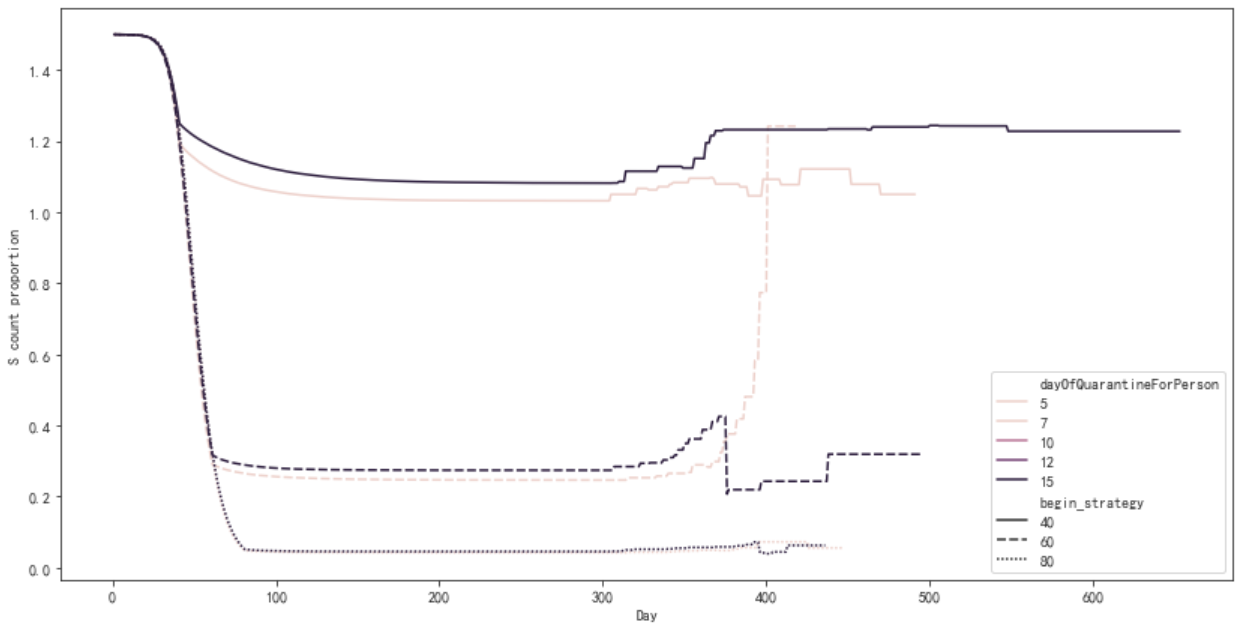
\includegraphics[width=5.5cm]{img/S}
                    %\caption{fig1}
                    }
                    \quad
                    \subfigure[E]{
                    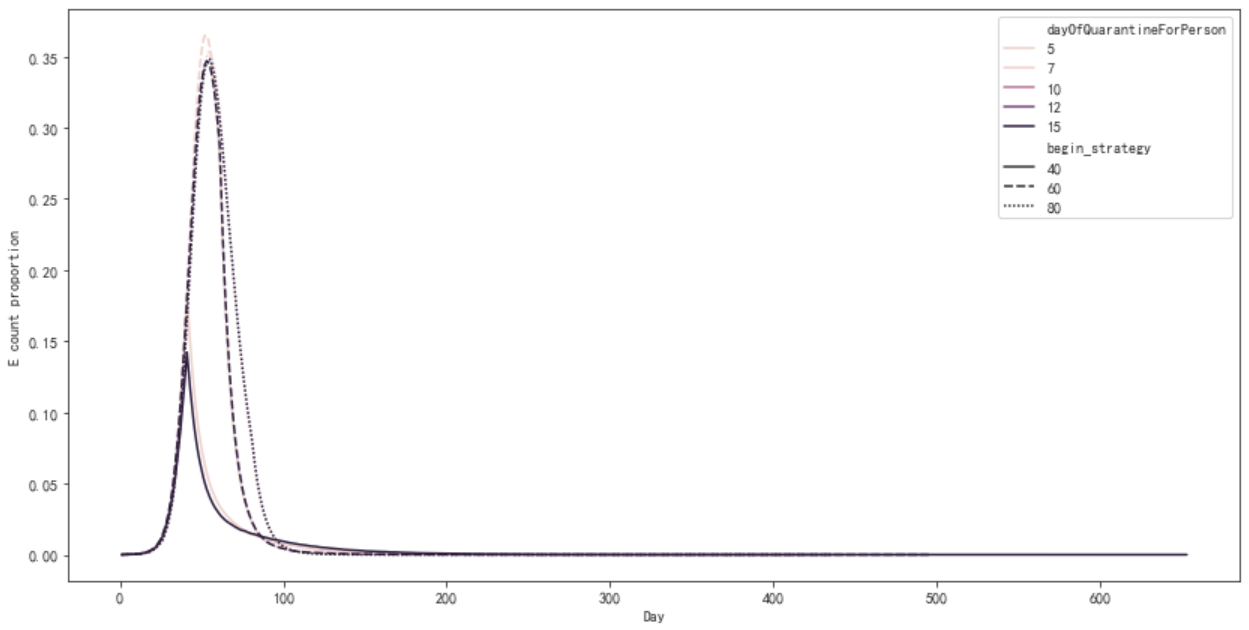
\includegraphics[width=5.5cm]{img/E.png}
                    }
                    \quad
                    \subfigure[A]{
                    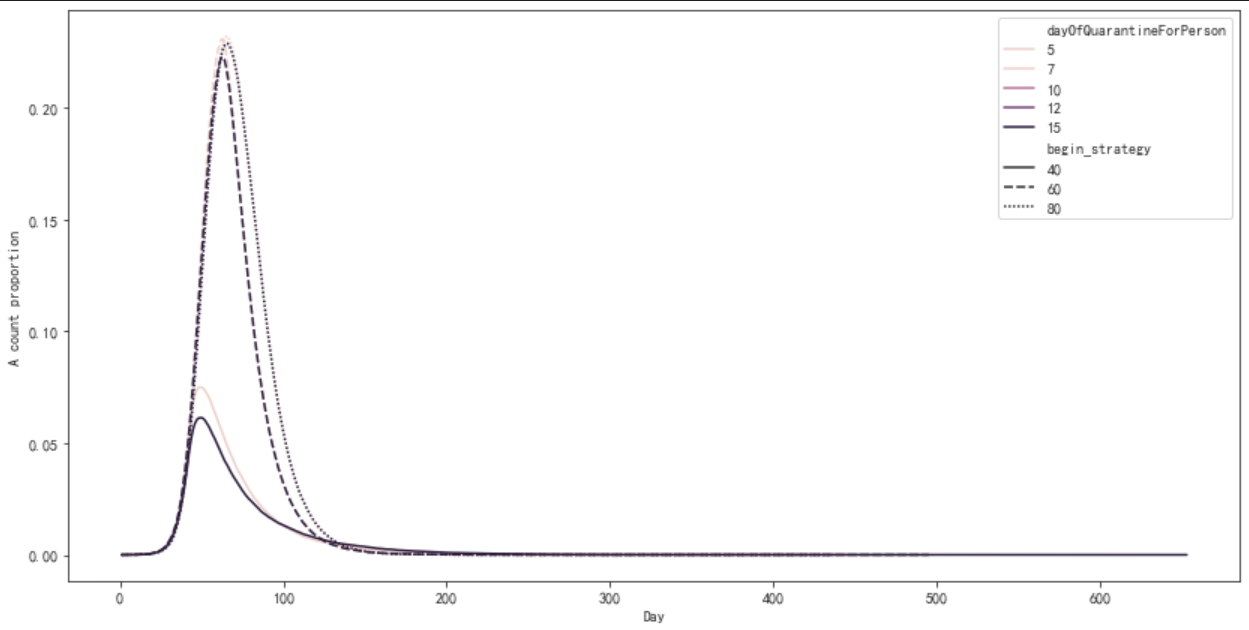
\includegraphics[width=5.5cm]{img/A.png}
                    }
                    \quad
                    \subfigure[I]{
                    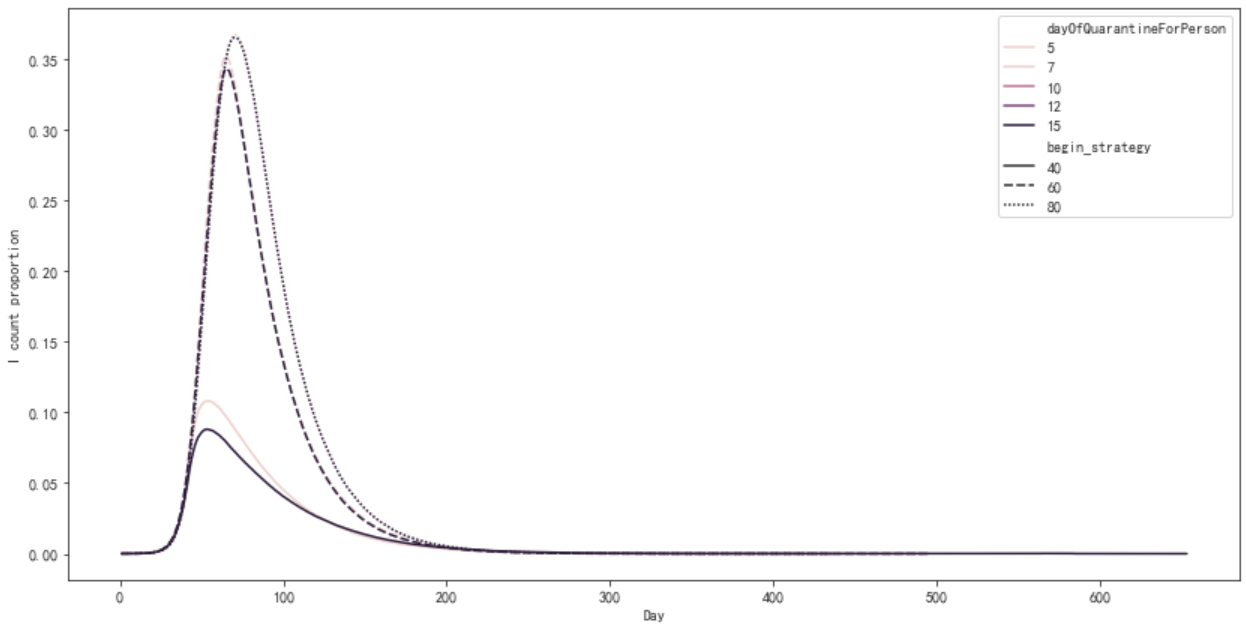
\includegraphics[width=5.5cm]{img/I.png}
                    }
                    \quad
                    \subfigure[R]{
                    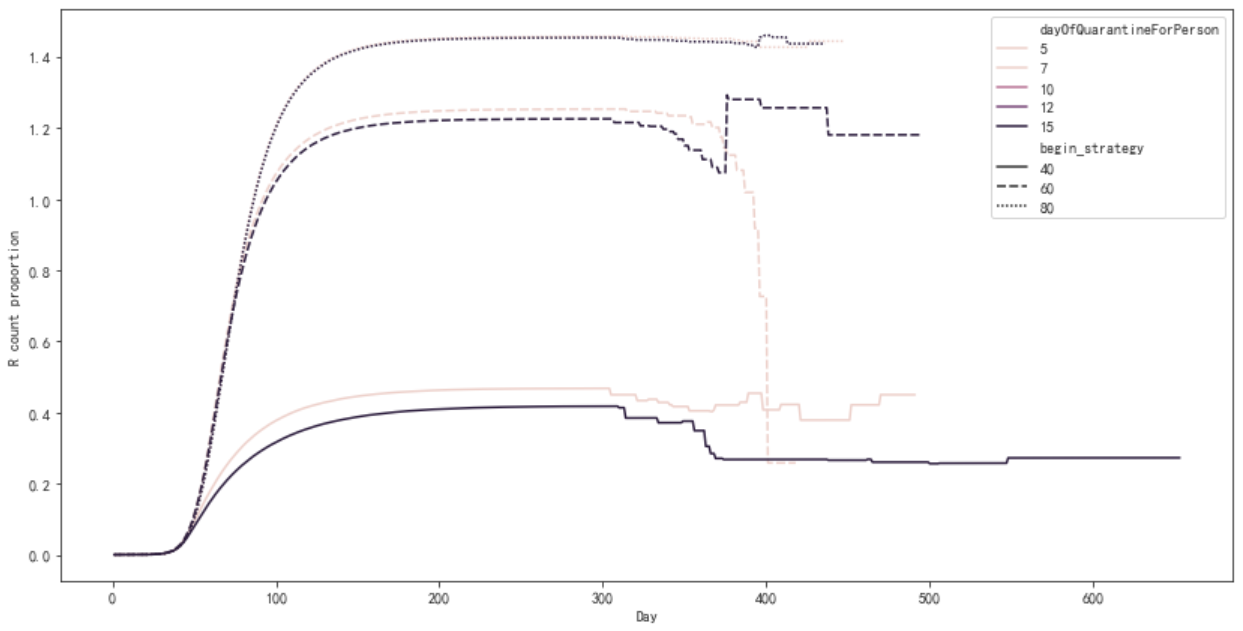
\includegraphics[width=5.5cm]{img/R}
                    }
                    \caption{各个状态人数占总人数}
                \end{figure}

                从图中可以看出,处于S状态和R状态图可以明显看到在iteration>300时,曲线的变化不像以往缓慢,S占比开始上升,而R开始下降,而在iteration>400时,
                S和R都开始出现垂直上升或下降或者暂缓不变的现象。于是,我们将S和R的占比画在同一幅图里,以观察他们的之间的关系。
                \begin{figure}[H]
                    \centering
                    \subfigure[7]{
                    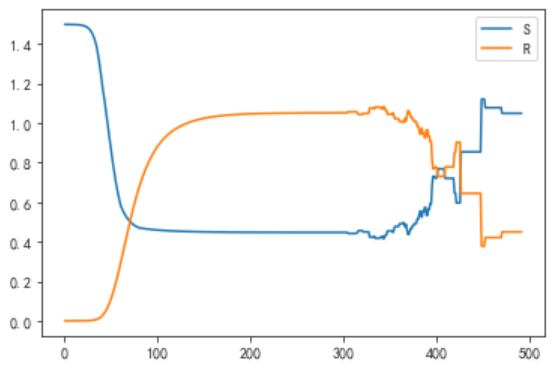
\includegraphics[width=5.5cm]{img/7}
                    %\caption{fig1}
                    }
                    \quad
                    \subfigure[14]{
                    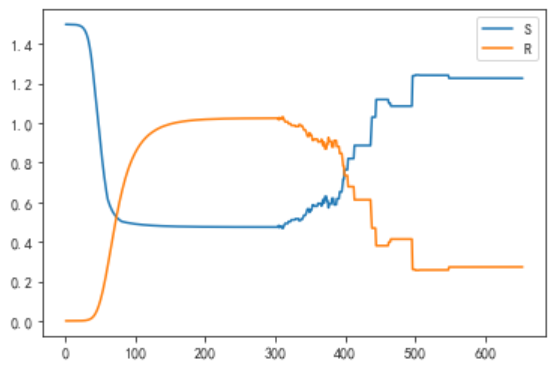
\includegraphics[width=5.5cm]{img/14}
                    }
                    \caption{处于S状态和R状态占比分析图}
                \end{figure}
                可以看到,S状态与R状态在dayOfQuarantineForPerson=7或dayOfQuarantineForPerson=14时都表现出对称性,目前未发现出现此现象的原因。
    \chapter{基于历史轨迹的区域检测}
    \chapter{基于图神经网络的区域检测推荐}


    
